\section{多層パーセプトロン}

%ニューラルネットワークとはニューロンとニューロン間のシナプスによる結合で形成される脳のネットワークを模した数理モデルである。入力層と出力層を持ち、シナプスの結合強度を変化させることで問題に最適なネットワークを構成することを目標とする。\par
%この説明は多層パーセプトロン
%また、入力層と出力層の間に隠れ層を加えて多層にし層間に活性化関数を用いて非線形分離を行うことで、複雑なネットワークを作ることができる。さらに、任意の活性化関数が微分可能であれば、誤差逆伝播法により損失関数を高速に求めることができる。\par

%ディープラーニングとは層をより深くしたニューラルネットワークを用いた機械学習の手法である。\par
%また、層を増やすと勾配の減衰による勾配消失や訓練データへの最適化による過学習などの問題が発生するが、前者の場合は活性化関数にReLU関数を用い後者の場合は汎化性能を測定することで避けることができる。\par

%以下、abst,intro,method,しか読んでないものがほとんど

\section{GAN}

\begin{figure}[h]
    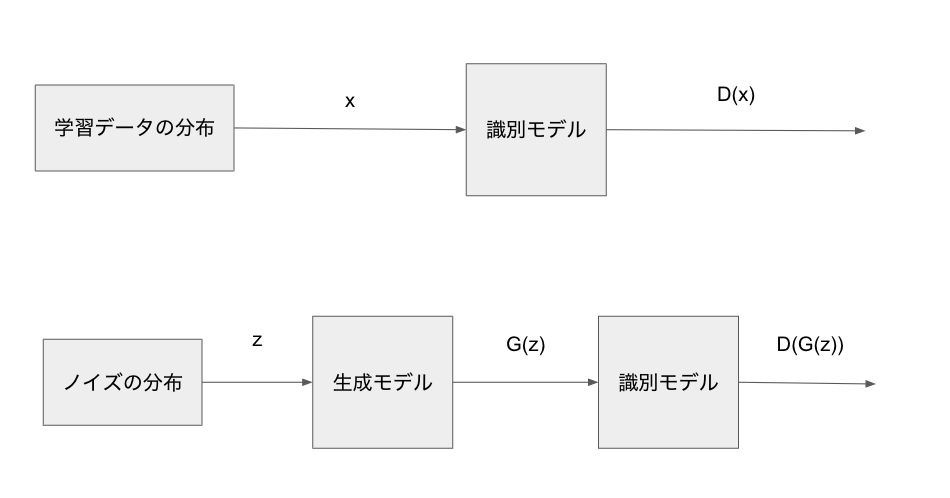
\includegraphics[width=10.0cm]{figure/GAN.png}
\end{figure}

GAN~(敵対的生成モデル)とは生成モデルと識別モデルが競合して学習を行うディープラーニングのモデルである。生成モデルは訓練データの分布を捉えようとし、識別モデルは訓練データである確率を推定する。\par
具体的には、訓練データ$x$の分布を$p_{data}$,生成モデルの入力のノイズ$z$の分布を$p_z$,ノイズ$z$を元にデータを生成する関数を$G$,生成モデルのデータではなく訓練データである確率を返す関数を$D$とした時、式\ref{eq:GAN}を生成モデルは最小化し識別モデルは最大化をすることを目標として学習を行う~\cite{GAN}。


\begin{align}
\label{eq:GAN}
    \mathbb{E}_{\boldsymbol{x} \sim p_{\text {data }}(\boldsymbol{x})}[\log D(\boldsymbol{x})]+\mathbb{E}_{\boldsymbol{z} \sim p_{\boldsymbol{z}}}(\boldsymbol{z})[\log (1-D(G(\boldsymbol{z})))]
\end{align}

\section{CGAN}

\begin{figure}[h]
    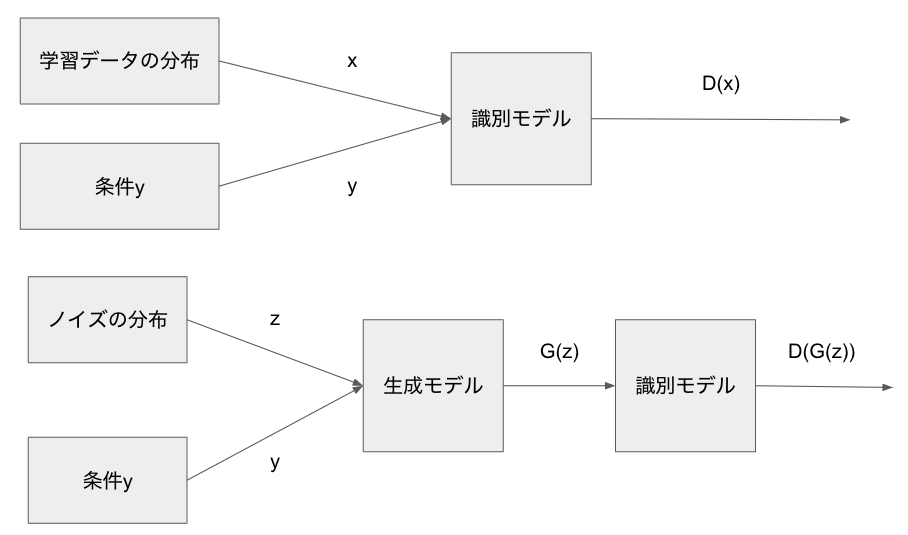
\includegraphics[width=10.0cm]{figure/CGAN.png}
\end{figure}

CGAN(条件付き敵対的生成モデル)とは条件付きのGANである。具体的には$y$という条件下で式\ref{eq:CGAN}を生成モデルは最小化し識別モデルは最大化をすることを目標として学習を行う\cite{CGAN}。\par
原著論文では訓練時にMNISTの数字のラベルを条件として与えることで特定の数字のラベルの画像を生成するモデルを実装している。


\begin{align}
    \label{eq:CGAN}
    \mathbb{E}_{\boldsymbol{x} \sim p_{\text {data }}(\boldsymbol{x})}[\log D(\boldsymbol{x} \mid \boldsymbol{y})]+\mathbb{E}_{\boldsymbol{z} \sim p_{z}(\boldsymbol{z})}[\log (1-D(G(\boldsymbol{z} \mid \boldsymbol{y})))]
\end{align}


\section{Pix2pix}

pix2pixとはある条件下で画像間の変換を行うGANである。先程のCGANを元にU-NetとPatachGANを組み合わせたネットワークになっている。\textcolor{red}{U-netとは…,PatchGANとは…。(ここは後々調べて書く)}\par
具体的には、画像$x$を条件として式\ref{eq:pix2pix3}を生成モデルは最小化し識別モデルは最大化をすることを目標として学習を行う\cite{pix2pix}。

\begin{align}
    \mathcal{L}_{cGAN}(G, D)=\mathbb{E}_{x, y}[\log D(x, y)]+\mathbb{E}_{x, z}[\log (1-D(x, G(x, z)))] \label{eq:pix2pix1}\\
    \mathcal{L}_{L 1}(G)=\mathbb{E}_{x, y, z}\left[\|y-G(x, z)\|_{1}\right] \label{peq:ix2pix2}\\
    \mathcal{L}_{c G A N}(G, D)+\lambda \mathcal{L}_{L 1}(G) \label{eq:pix2pix3}
\end{align}

%CycleGAN(検討)
%自己回帰モデル(検討)
%https://ja.wikipedia.org/wiki/%E8%87%AA%E5%B7%B1%E5%9B%9E%E5%B8%B0%E3%83%A2%E3%83%87%E3%83%AB
%Wavenet(検討)
%スペクトログラム(検討)